% Options for packages loaded elsewhere
\PassOptionsToPackage{unicode}{hyperref}
\PassOptionsToPackage{hyphens}{url}
\PassOptionsToPackage{dvipsnames,svgnames,x11names}{xcolor}
%
\documentclass[
  letterpaper,
  DIV=11,
  numbers=noendperiod]{scrartcl}

\usepackage{amsmath,amssymb}
\usepackage{iftex}
\ifPDFTeX
  \usepackage[T1]{fontenc}
  \usepackage[utf8]{inputenc}
  \usepackage{textcomp} % provide euro and other symbols
\else % if luatex or xetex
  \usepackage{unicode-math}
  \defaultfontfeatures{Scale=MatchLowercase}
  \defaultfontfeatures[\rmfamily]{Ligatures=TeX,Scale=1}
\fi
\usepackage{lmodern}
\ifPDFTeX\else  
    % xetex/luatex font selection
\fi
% Use upquote if available, for straight quotes in verbatim environments
\IfFileExists{upquote.sty}{\usepackage{upquote}}{}
\IfFileExists{microtype.sty}{% use microtype if available
  \usepackage[]{microtype}
  \UseMicrotypeSet[protrusion]{basicmath} % disable protrusion for tt fonts
}{}
\makeatletter
\@ifundefined{KOMAClassName}{% if non-KOMA class
  \IfFileExists{parskip.sty}{%
    \usepackage{parskip}
  }{% else
    \setlength{\parindent}{0pt}
    \setlength{\parskip}{6pt plus 2pt minus 1pt}}
}{% if KOMA class
  \KOMAoptions{parskip=half}}
\makeatother
\usepackage{xcolor}
\setlength{\emergencystretch}{3em} % prevent overfull lines
\setcounter{secnumdepth}{-\maxdimen} % remove section numbering
% Make \paragraph and \subparagraph free-standing
\makeatletter
\ifx\paragraph\undefined\else
  \let\oldparagraph\paragraph
  \renewcommand{\paragraph}{
    \@ifstar
      \xxxParagraphStar
      \xxxParagraphNoStar
  }
  \newcommand{\xxxParagraphStar}[1]{\oldparagraph*{#1}\mbox{}}
  \newcommand{\xxxParagraphNoStar}[1]{\oldparagraph{#1}\mbox{}}
\fi
\ifx\subparagraph\undefined\else
  \let\oldsubparagraph\subparagraph
  \renewcommand{\subparagraph}{
    \@ifstar
      \xxxSubParagraphStar
      \xxxSubParagraphNoStar
  }
  \newcommand{\xxxSubParagraphStar}[1]{\oldsubparagraph*{#1}\mbox{}}
  \newcommand{\xxxSubParagraphNoStar}[1]{\oldsubparagraph{#1}\mbox{}}
\fi
\makeatother


\providecommand{\tightlist}{%
  \setlength{\itemsep}{0pt}\setlength{\parskip}{0pt}}\usepackage{longtable,booktabs,array}
\usepackage{calc} % for calculating minipage widths
% Correct order of tables after \paragraph or \subparagraph
\usepackage{etoolbox}
\makeatletter
\patchcmd\longtable{\par}{\if@noskipsec\mbox{}\fi\par}{}{}
\makeatother
% Allow footnotes in longtable head/foot
\IfFileExists{footnotehyper.sty}{\usepackage{footnotehyper}}{\usepackage{footnote}}
\makesavenoteenv{longtable}
\usepackage{graphicx}
\makeatletter
\def\maxwidth{\ifdim\Gin@nat@width>\linewidth\linewidth\else\Gin@nat@width\fi}
\def\maxheight{\ifdim\Gin@nat@height>\textheight\textheight\else\Gin@nat@height\fi}
\makeatother
% Scale images if necessary, so that they will not overflow the page
% margins by default, and it is still possible to overwrite the defaults
% using explicit options in \includegraphics[width, height, ...]{}
\setkeys{Gin}{width=\maxwidth,height=\maxheight,keepaspectratio}
% Set default figure placement to htbp
\makeatletter
\def\fps@figure{htbp}
\makeatother

\KOMAoption{captions}{tableheading}
\makeatletter
\@ifpackageloaded{tcolorbox}{}{\usepackage[skins,breakable]{tcolorbox}}
\@ifpackageloaded{fontawesome5}{}{\usepackage{fontawesome5}}
\definecolor{quarto-callout-color}{HTML}{909090}
\definecolor{quarto-callout-note-color}{HTML}{0758E5}
\definecolor{quarto-callout-important-color}{HTML}{CC1914}
\definecolor{quarto-callout-warning-color}{HTML}{EB9113}
\definecolor{quarto-callout-tip-color}{HTML}{00A047}
\definecolor{quarto-callout-caution-color}{HTML}{FC5300}
\definecolor{quarto-callout-color-frame}{HTML}{acacac}
\definecolor{quarto-callout-note-color-frame}{HTML}{4582ec}
\definecolor{quarto-callout-important-color-frame}{HTML}{d9534f}
\definecolor{quarto-callout-warning-color-frame}{HTML}{f0ad4e}
\definecolor{quarto-callout-tip-color-frame}{HTML}{02b875}
\definecolor{quarto-callout-caution-color-frame}{HTML}{fd7e14}
\makeatother
\makeatletter
\@ifpackageloaded{caption}{}{\usepackage{caption}}
\AtBeginDocument{%
\ifdefined\contentsname
  \renewcommand*\contentsname{Table of contents}
\else
  \newcommand\contentsname{Table of contents}
\fi
\ifdefined\listfigurename
  \renewcommand*\listfigurename{List of Figures}
\else
  \newcommand\listfigurename{List of Figures}
\fi
\ifdefined\listtablename
  \renewcommand*\listtablename{List of Tables}
\else
  \newcommand\listtablename{List of Tables}
\fi
\ifdefined\figurename
  \renewcommand*\figurename{Figure}
\else
  \newcommand\figurename{Figure}
\fi
\ifdefined\tablename
  \renewcommand*\tablename{Table}
\else
  \newcommand\tablename{Table}
\fi
}
\@ifpackageloaded{float}{}{\usepackage{float}}
\floatstyle{ruled}
\@ifundefined{c@chapter}{\newfloat{codelisting}{h}{lop}}{\newfloat{codelisting}{h}{lop}[chapter]}
\floatname{codelisting}{Listing}
\newcommand*\listoflistings{\listof{codelisting}{List of Listings}}
\makeatother
\makeatletter
\makeatother
\makeatletter
\@ifpackageloaded{caption}{}{\usepackage{caption}}
\@ifpackageloaded{subcaption}{}{\usepackage{subcaption}}
\makeatother

\ifLuaTeX
  \usepackage{selnolig}  % disable illegal ligatures
\fi
\usepackage{bookmark}

\IfFileExists{xurl.sty}{\usepackage{xurl}}{} % add URL line breaks if available
\urlstyle{same} % disable monospaced font for URLs
\hypersetup{
  pdftitle={Module 2: Lab Instructions},
  colorlinks=true,
  linkcolor={blue},
  filecolor={Maroon},
  citecolor={Blue},
  urlcolor={Blue},
  pdfcreator={LaTeX via pandoc}}


\title{Module 2: Lab Instructions}
\author{}
\date{}

\begin{document}
\maketitle


\subsection{Purpose}\label{purpose}

The purpose of today's lab is to: (1) visualize the Central Limit
Theorem, and (2) practice the steps of Null Hypothesis Significance
Testing (NHST).

\subsection{Access the Starter Files for Module
2}\label{access-the-starter-files-for-module-2}

\begin{itemize}
\item
  Go to \url{posit.cloud} and then \textbf{navigate to the course
  workspace} via the left sidebar.

  \begin{itemize}
  \tightlist
  \item
    Look for the course workspace called ``Statistical Methods Spring
    2025''
  \end{itemize}
\item
  Open the project titled \textbf{Module 2} This module contains the
  starter files that you will use for this lab and for your homework.
\end{itemize}

\subsection{Starter Files}\label{starter-files}

In the Files pane you should see these two R Notebooks:

\begin{itemize}
\tightlist
\item
  mod-02-lab-starter.qmd
\item
  mod-02-hw-starter.qmd
\end{itemize}

Go ahead and open up \texttt{mod-02-lab-starter.qmd}. This is your
``starter file'' for today's lab. You will build upon this document as
you work on the exercises in this lab session.

\subsection{Step 1: Check that the file
Renders!}\label{step-1-check-that-the-file-renders}

Click the button called ``Render'' (circled in the image below) and then
double check to see that your document rendered in the \textbf{Viewer}
pane. It is always a good idea to occasionally check that the document
still renders correctly after making changes.

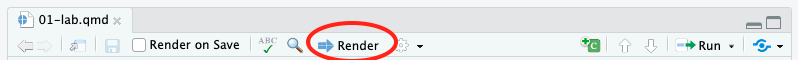
\includegraphics{images/render.png}

\subsection{Step 2: Load Packages}\label{step-2-load-packages}

Today, we'll be using the following packages:

\begin{itemize}
\tightlist
\item
  \textbf{tidyverse}: a collection of packages for doing data analysis
  in a ``tidy'' way
\item
  \textbf{infer}: a package designed for statistical inference, we will
  be using it to generate ``sample'' datasets
\item
  \textbf{knitr}: a package that supports the integration of code into
  text documents, we will be using it today to create a table
\end{itemize}

Please load these packages using the \texttt{library()} function. If the
packages don't load, you may need to \texttt{install.packages()} first.

\subsection{Step 3: Read in the Data}\label{step-3-read-in-the-data}

The data we will use in Module 2 is from the Gapminder Foundation, a
non-profit collects data about social, economic, and environmental
development at local, national, and global levels. The data we will use
today were collected in 2015.

Read in the data using the \texttt{read\_csv()} function. Name the data
``gapminder\_2015''

Now, use the \texttt{View()} function to take a look at your data.

\subsection{Exercise 1:}\label{exercise-1}

For this first exercise, we are going to generate 10000 random samples
of different sizes (5, 30, and 100) from a skewed distribution. For each
sample, we will calculate the mean. Then, we will plot those 1000 means
to examine the resulting sampling distributions. We will use the
(depressing, sorry!) infant\_mortality variable in the gapminder data.

Compare the three plots, what does this show?

\subsection{Exercise 2:}\label{exercise-2}

Now, let's practice the steps of Null Hypothesis Significance Testing
(NHST).

\begin{tcolorbox}[enhanced jigsaw, opacityback=0, colbacktitle=quarto-callout-note-color!10!white, colback=white, toptitle=1mm, title=\textcolor{quarto-callout-note-color}{\faInfo}\hspace{0.5em}{Note}, left=2mm, colframe=quarto-callout-note-color-frame, coltitle=black, bottomtitle=1mm, titlerule=0mm, leftrule=.75mm, toprule=.15mm, rightrule=.15mm, bottomrule=.15mm, arc=.35mm, opacitybacktitle=0.6, breakable]

There is no data to read in for this exercise.

\end{tcolorbox}

A psychologist is investigating the impact of a new mindfulness
meditation technique on stress levels. It is known that the average
stress score on a well-validated scale is 75 for the general population.

The psychologist recruits 25 participants to undergo the mindfulness
meditation program for 8 weeks. After the program, the participants
complete the standardized stress scale. The sample of participants has
an average stress score of 68 with a standard deviation of 12.

\textbf{Step 1:} State the null and alternative hypotheses. Use
\emph{non-directional} hypotheses.

H\textsubscript{0}:

H\textsubscript{1}:

\textbf{Step 2:} Choose your alpha level. If you choose not to use
\(\alpha\) = .05, provide a justification.

\(\alpha\):

\textbf{Step 3:} Collect your data.

We're going to pretend we already did this!

Restating from above: Our sample mean is 68 and sample standard
deviation is 12. The population mean is 75.

\(\bar{x}\) = 68

\emph{s} = 12

\(\mu\) = 75

\textbf{Step 4:} Define the mean and SEM for the sampling distribution.
Estimate the population mean and sd from your data, calculate the SEM.
Report the SEM.

\emph{SEM} = \(\sigma\) / \(\sqrt{n}\)

\begin{tcolorbox}[enhanced jigsaw, opacityback=0, colbacktitle=quarto-callout-note-color!10!white, colback=white, toptitle=1mm, title=\textcolor{quarto-callout-note-color}{\faInfo}\hspace{0.5em}{Note}, left=2mm, colframe=quarto-callout-note-color-frame, coltitle=black, bottomtitle=1mm, titlerule=0mm, leftrule=.75mm, toprule=.15mm, rightrule=.15mm, bottomrule=.15mm, arc=.35mm, opacitybacktitle=0.6, breakable]

Note: While we are calculating these statistics for practice, and to
generate a confidence interval, we will use a t-distribution to generate
the \emph{exact} p-value for our observed data. You should always report
the exact p-value if you can unless it's under .001. In that case, you
would report \emph{p} \textless{} .001.

\end{tcolorbox}

\textbf{Step 5:} Determine the probability of your data or more extreme
under the null distribution. Calculate the t-statistic and then generate
a p-value using the \texttt{pt()} function.

\emph{t} = (\(\bar{x}\) - \(\mu\)) / \emph{SEM}

\textbf{Step 6:} Compare your probability (p-value) to your alpha level
and decide whether to reject or retain the null hypothesis.

\textbf{Step 7:} Write up your results summary. Make sure to include a
Confidence Interval around your estimate of the mean.

95\% CI = \(\bar{x}\) ±(1.96 x SEM)

Make sure to include the following in your results summary:

\begin{itemize}
\tightlist
\item
  A brief statement about what you tested.
\item
  Descriptive statistics for your sample(s), including the confidence
  intervall around your estimate.
\item
  A statement of the direction of the effect.
\item
  Descriptives for the value or group you are comparing your sample to.
\item
  Results of the statistical test you performed, written in APA Style
  (including statistic and p-value).
\item
  A clear statement about what you found.
\end{itemize}

\begin{tcolorbox}[enhanced jigsaw, opacityback=0, colbacktitle=quarto-callout-note-color!10!white, colback=white, toptitle=1mm, title=\textcolor{quarto-callout-note-color}{\faInfo}\hspace{0.5em}{Note}, left=2mm, colframe=quarto-callout-note-color-frame, coltitle=black, bottomtitle=1mm, titlerule=0mm, leftrule=.75mm, toprule=.15mm, rightrule=.15mm, bottomrule=.15mm, arc=.35mm, opacitybacktitle=0.6, breakable]

The items listed above do not need to be included in this exact order.

\end{tcolorbox}

We examined the effect of an 8-week mindfulness meditation program on
stress levels. The average score of participants after the program
(\emph{M} = 68, 95\%CI {[}63.3, 72.7{]}, \emph{SD} = 12) was
significantly higher than the population average, (\(\mu\) = 75),
\emph{t}(24) = -2.92, \emph{p} = 0.008. This finding suggests that the
mindfulness meditation program has a significant impact on reducing
stress levels in participants.

\subsection{Consider the following alternative scenarios. What would you
conclude?}\label{consider-the-following-alternative-scenarios.-what-would-you-conclude}

If observed sample mean was 72, the t statistic would be -1.25 and
p-value would be 0.22. What do you conclude?

If the observed sample mean was 82, the t statistic would be 2.92 and
p-value would be .008. What do you conclude?

\subsection{Render your document.}\label{render-your-document.}

Note: You do not need to submit your lab, but you will need to submit a
rendered PDF version of your homework to ``Module 2: Homework
Submission'' on Canvas.

\begin{itemize}
\tightlist
\item
  At the top of the .qmd file, change ``format: html'' to ``format:
  pdf''
\item
  Click ``Render'' at the top of the document
\item
  Your document will open in a browser tab
\item
  If your document opens in the ``Viewer'' pane, click the ``sidebar''
  button (circled in image below)
\end{itemize}

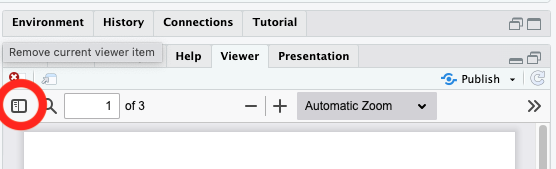
\includegraphics{images/sidebar.png}

\begin{itemize}
\tightlist
\item
  If you get a popup warning, click ``Try Again'' (may be specific to
  Mac)
\item
  Click the ``Save'' icon on the top right (circled in the image below)
\end{itemize}


\includegraphics{images/save_pdf.png}

\begin{itemize}
\tightlist
\item
  Save wherever you keep your class documents and upload your file to
  Canvas
\end{itemize}

\begin{center}\rule{0.5\linewidth}{0.5pt}\end{center}




\end{document}
